%% Báo cáo tiến độ — 2 papers: CRSD/Climate (Paper A) + PGG/Punishment (Paper B)
%% Trục chung: behavioural validity của LLM agents như "silicon samples".
%% Biên dịch: xelatex (hỗ trợ tiếng Việt + font hệ thống), chạy 2 lần.
%%   xelatex LLM_Cooperation_Talk.tex

\documentclass[aspectratio=169,11pt]{beamer}

\usepackage{fontspec}
\usepackage{booktabs}
\usepackage{colortbl}
\usepackage{array}
\usepackage{tikz}
\usetikzlibrary{positioning,arrows.meta}
\usepackage{ragged2e}

\usefonttheme{professionalfonts}
\setbeamertemplate{navigation symbols}{}
\graphicspath{{figures/}}

%% ---------- Font (Vietnamese-capable, modern) ----------
\setsansfont{Segoe UI}[
  BoldFont      = {Segoe UI Semibold},
  ItalicFont    = {Segoe UI Italic},
  BoldItalicFont= {Segoe UI Semibold Italic}
]
\setmonofont{Consolas}
\renewcommand{\familydefault}{\sfdefault}

%% ---------- Color palette ----------
\definecolor{primary}{HTML}{0E4C5A}     % deep teal (frame)
\definecolor{primaryDark}{HTML}{082F39}
\definecolor{accent}{HTML}{E84855}      % coral red (human / risk / antisocial)
\definecolor{amber}{HTML}{E8A04B}       % amber accent
\definecolor{paperA}{HTML}{2E6E8E}      % blue  -> Paper A (climate)
\definecolor{paperB}{HTML}{8E4585}      % plum  -> Paper B (punishment)
\definecolor{good}{HTML}{2E8B6F}        % green (prosocial / reproduced)
\definecolor{ink}{HTML}{1F2A30}
\definecolor{mute}{HTML}{5B6B72}
\definecolor{lightbg}{HTML}{F2F6F7}
\definecolor{rule}{HTML}{CBD8DC}

%% ---------- Beamer color assignments ----------
\setbeamercolor{normal text}{fg=ink}
\setbeamercolor{frametitle}{fg=white,bg=primary}
\setbeamercolor{title}{fg=white}
\setbeamercolor{structure}{fg=primary}
\setbeamercolor{itemize item}{fg=primary}
\setbeamercolor{itemize subitem}{fg=amber}
\setbeamercolor{block title}{fg=white,bg=primary}
\setbeamercolor{block body}{fg=ink,bg=lightbg}
\setbeamercolor{alerted text}{fg=accent}

\setbeamerfont{frametitle}{series=\bfseries,size=\large}
\setbeamerfont{title}{series=\bfseries,size=\LARGE}
\setbeamerfont{block title}{series=\bfseries}
\setbeamerfont{footline}{size=\scriptsize}

%% ---------- Frame title bar ----------
\setbeamertemplate{frametitle}{%
  \nointerlineskip%
  \begin{beamercolorbox}[wd=\paperwidth,ht=2.5em,dp=0.9em,leftskip=0.7cm,rightskip=0.7cm]{frametitle}%
    \usebeamerfont{frametitle}\insertframetitle%
  \end{beamercolorbox}%
}

%% ---------- Itemize markers ----------
\setbeamertemplate{itemize item}{\raisebox{0.12em}{\rule{0.55em}{0.55em}}}
\setbeamertemplate{itemize subitem}{\raisebox{0.1em}{\small\textcolor{amber}{\rule{0.45em}{0.45em}}}}
\setbeamertemplate{itemize subsubitem}{\textcolor{mute}{--}}

%% ---------- Footline ----------
\setbeamertemplate{footline}{%
  \leavevmode%
  \hbox{%
    \begin{beamercolorbox}[wd=.30\paperwidth,ht=2.6ex,dp=1.1ex,leftskip=0.7cm]{}%
      \color{mute}\scriptsize 2 papers · LLM agents
    \end{beamercolorbox}%
    \begin{beamercolorbox}[wd=.54\paperwidth,ht=2.6ex,dp=1.1ex,center]{}%
      \color{mute}\scriptsize Behavioural validity của LLM trong trò chơi hợp tác
    \end{beamercolorbox}%
    \begin{beamercolorbox}[wd=.16\paperwidth,ht=2.6ex,dp=1.1ex,rightskip=0.7cm]{}%
      \hfill\color{primary}\scriptsize\bfseries \insertframenumber\,/\,\inserttotalframenumber
    \end{beamercolorbox}%
  }%
}

\setbeamertemplate{itemize/enumerate body begin}{\justifying}
\setlength{\parskip}{2pt}

%% ---------- Helper commands ----------
\newcommand{\hl}[1]{\textbf{\textcolor{primary}{#1}}}
\newcommand{\hlr}[1]{\textbf{\textcolor{accent}{#1}}}
\newcommand{\hlg}[1]{\textbf{\textcolor{good}{#1}}}
\newcommand{\pA}[1]{\textbf{\textcolor{paperA}{#1}}}
\newcommand{\pB}[1]{\textbf{\textcolor{paperB}{#1}}}
\newcommand{\pAt}[1]{{\color{amber}\bfseries #1}}
\newcommand{\pBt}[1]{{\color{amber}\bfseries #1}}
\providecommand{\euro}{€}
\newcommand{\eur}{\euro}

%% ---------- Section divider ----------
\AtBeginSection[]{%
  \begin{frame}[plain,noframenumbering]
    \begin{tikzpicture}[remember picture,overlay]
      \fill[primary] (current page.south west) rectangle (current page.north east);
      \fill[amber] ([yshift=-3.2cm]current page.west) rectangle ([yshift=-3.4cm]current page.east);
    \end{tikzpicture}
    \vfill
    \begin{center}
      {\color{white!75!primary}\large\bfseries Phần \insertsectionnumber}\\[0.4em]
      {\color{white}\Huge\bfseries \insertsectionhead}
    \end{center}
    \vfill
  \end{frame}
}

%% ================= METADATA =================
\title{LLM agents có phải là ``silicon samples'' hợp lệ?}
\author{Nghiên cứu sinh — Game Theory}
\date{\today}

\begin{document}

%% ================= SECTION 2 : PAPER A =================
\section{Paper A — Collective-risk climate dilemma}

\begin{frame}{\pA{Paper A} — Trò chơi CRSD (Milinski 2008)}
  \begin{columns}[T]
    \begin{column}{0.56\textwidth}
      \begin{itemize}
        \item \hl{6 người chơi}, mỗi người vốn \eur40, chơi \hl{10 vòng}.
        \item Mỗi vòng góp \hl{\eur0 / \eur2 / \eur4} vào ``quỹ khí hậu''.
        \item Mục tiêu nhóm: tích lũy \hl{\eur120}; không đạt $\Rightarrow$ \hlr{xổ số}: x.suất $p$ mọi người \hlr{mất sạch}.
        \item Biến chẩn đoán: \pA{$p \in \{90\%, 50\%, 10\%\}$}; tối đa \eur240.
      \end{itemize}
      \vspace{0.15cm}
      \begin{block}{Đặc trưng hành vi ở con người}
        $p$ giảm $\Rightarrow$ đầu tư \hlr{giảm mạnh} (\eur118$\to$92$\to$73; ANOVA $F=13.78$).
      \end{block}
    \end{column}
    \begin{column}{0.44\textwidth}
      \centering
      \begin{tikzpicture}[scale=1.0]
        \draw[->,thick,mute] (-0.2,0) -- (4.6,0) node[right,font=\scriptsize]{$p$ giảm $\to$};
        \draw[->,thick,mute] (0,-0.1) -- (0,3.3) node[above,font=\scriptsize]{Đầu tư (\eur)};
        \filldraw[accent] (0.5,0) rectangle (1.2,2.95);
        \filldraw[accent!75] (1.9,0) rectangle (2.6,2.30);
        \filldraw[accent!55] (3.3,0) rectangle (4.0,1.83);
        \node[font=\scriptsize,white] at (0.85,1.5) {118};
        \node[font=\scriptsize,white] at (2.25,1.2) {92};
        \node[font=\scriptsize,white] at (3.65,0.95) {73};
        \node[font=\scriptsize,mute] at (0.85,-0.3) {90\%};
        \node[font=\scriptsize,mute] at (2.25,-0.3) {50\%};
        \node[font=\scriptsize,mute] at (3.65,-0.3) {10\%};
        \node[font=\scriptsize\bfseries,primary] at (2.3,3.2) {Con người: dốc xuống};
      \end{tikzpicture}\\[0.2cm]
      {\scriptsize\color{mute}Milinski et al. 2008, PNAS}
    \end{column}
  \end{columns}
\end{frame}

\begin{frame}{\pA{A1} — Over-cooperation ở mọi mức rủi ro}
  \centering
  \renewcommand{\arraystretch}{1.2}
  \begin{tabular}{l c c c}
    \toprule
    \textbf{Người chơi} & \textbf{$p=90\%$} & \textbf{$p=50\%$} & \textbf{$p=10\%$}\\
    \midrule
    \rowcolor{accent!12} Con người \footnotesize(Milinski) & 118.2\ \footnotesize(50\%) & 92.2\ \footnotesize(10\%) & 73.0\ \footnotesize(0\%)\\
    Qwen2.5-7B   & \hl{183.0}\ \footnotesize(100\%) & \hl{186.6}\ \footnotesize(100\%) & \hl{181.0}\ \footnotesize(100\%)\\
    Gemma-2-9B   & \hl{168.2}\ \footnotesize(100\%) & \hl{162.8}\ \footnotesize(100\%) & \hl{158.0}\ \footnotesize(100\%)\\
    Llama-3.1-8B & \hl{177.4}\ \footnotesize(100\%) & \hl{165.2}\ \footnotesize(100\%) & \hl{170.0}\ \footnotesize(100\%)\\
    \bottomrule
  \end{tabular}\\[0.25em]
  {\footnotesize\color{mute}Final group total \eur\ (tỉ lệ đạt target). Target $=$ \eur120; tối đa khả thi $=$ \eur240.}

  \vspace{0.4cm}
  \begin{columns}[T]
    \begin{column}{0.5\textwidth}
      \begin{itemize}\footnotesize
        \item Cả 3 model đạt target \hl{100\% mọi mức risk}.
        \item Đầu tư \hl{\eur158--187} ($\approx$66--78\% trần \eur240).
      \end{itemize}
    \end{column}
    \begin{column}{0.5\textwidth}
      \begin{itemize}\footnotesize
        \item $\sim$\hl{6/6} fair-sharers vs 1--3 ở người.
        \item Mọi contrast LLM--người đều \hl{significant}.
      \end{itemize}
    \end{column}
  \end{columns}
\end{frame}

\begin{frame}{\pA{A2 (QUYẾT ĐỊNH)} — Vô cảm với rủi ro thảm họa}
  \centering
  
\includegraphics[width=0.84\textwidth]{fig1_risk.pdf}\\[0.45em]
  {\small\textbf{\textcolor{accent}{Người giảm dốc khi rủi ro giảm — cả 3 model gần như PHẲNG, đều vượt \eur120.}}}\\[0.3em]
  {\footnotesize\color{mute}ANOVA $F$: \hl{13.78} (người) vs \hl{1.76 / 2.23 / 3.64} \;\textbullet\; TOST $p\le.014$ \;\textbullet\; $\mathrm{BF}_{01}$ 4.8 / 3.0 (Llama equivocal)}
\end{frame}

\begin{frame}{\pA{A3} — Hợp tác do disposition chi phối, bất biến qua ngôn ngữ}
  \centering
  
\includegraphics[width=0.84\textwidth]{fig2_moderators.pdf}\\[0.45em]
  {\small\textbf{\textcolor{accent}{Đổi 1 câu disposition: selfish $\to$ 0\% thành công. Nội dung bất biến qua 5 ngôn ngữ.}}}\\[0.3em]
  {\footnotesize\color{mute}Selfish 0\% (Qwen,Gemma) / 27\% (Llama) \;\textbullet\; risk-averse 73--93\% \;\textbullet\; \hl{5 ngôn ngữ đều $>$\eur120}}
\end{frame}

%% ================= SECTION 3 : PAPER B =================
\section{Paper B — Public-goods game với trừng phạt}

\begin{frame}{\pB{Paper B} — PGG với trừng phạt (Herrmann 2008)}
  \begin{columns}[T]
    \begin{column}{0.56\textwidth}
      \begin{itemize}
        \item \hl{4 người chơi} (partner), \hl{10 vòng}; mỗi vòng nhận \hl{20 token}.
        \item Góp vào quỹ chung, \emph{MPCR} $=0.4$ (mỗi token góp $\to$ 0.4 cho cả 4).
        \item \hl{2 treatment}: N (chỉ góp) vs \pB{P} (thêm \hl{trừng phạt tốn kém}).
        \begin{itemize}
          \item Trả 1 token để trừ 3 token của người khác (tỉ lệ 1:3).
        \end{itemize}
        \item Phân loại: trừng phạt người góp \emph{ít hơn} $=$ \hlg{prosocial}; góp \emph{bằng/nhiều hơn} $=$ \hlr{antisocial}.
      \end{itemize}
    \end{column}
    \begin{column}{0.44\textwidth}
      \begin{block}{2 đặc trưng chẩn đoán ở người}
        \begin{enumerate}\small
          \item \pB{Trừng phạt NÂNG hợp tác} (P$-$N $\approx +4.3$ token).
          \item \pB{Cấu trúc xuyên văn hóa}: antisocial punishment $\leftrightarrow$ hợp tác có $\rho\approx\hlr{-0.90}$ qua 16 xã hội.
        \end{enumerate}
      \end{block}
      \vspace{0.1cm}
      {\footnotesize\color{mute}16 personas thành phố trung lập (Boston\ldots Riyadh, Athens), không gán định kiến hành vi.}
    \end{column}
  \end{columns}
\end{frame}

\begin{frame}{\pB{B1} — Góp hào phóng \& trừng phạt, nhưng đa số là antisocial}
  \centering
  \renewcommand{\arraystretch}{1.2}
  \begin{tabular}{l c c c c}
    \toprule
    \textbf{Người chơi} & \textbf{Góp N} & \textbf{Góp P} & \textbf{$\Delta$ (P$-$N)} & \textbf{\% antisocial}\\
    \midrule
    \rowcolor{accent!12} Con người \footnotesize(Herrmann) & 8.6 & 12.9 & \hlg{$+4.3$} & \footnotesize thiểu số$^*$\\
    Qwen2.5-7B   & 14.26 & 13.90 & \hlr{$-0.36$}\ \footnotesize($p$=.71) & \hlr{59\%}\\
    Gemma-2-9B   & 13.41 & 9.86  & \hlr{$-3.55$}\ \footnotesize($p$<.001) & \hlr{55\%}\\
    Llama-3.1-8B & 10.67 & 10.75 & \hlr{$+0.08$}\ \footnotesize($p$=.91) & \hlr{54\%}\\
    \bottomrule
  \end{tabular}\\[0.25em]
  {\footnotesize\color{mute}Đóng góp trung bình /20 token. $^*$Ở người: antisocial là thiểu số ở pool phương Tây, nhưng \emph{cao} ở một số xã hội khác — chính là biến thiên xuyên văn hóa.}

  \vspace{0.4cm}
  \begin{itemize}\footnotesize
    \item Baseline N: cả 3 model \hl{trên mức người} (8.6); model \hl{có} góp \& \hl{có} trừng phạt.
    \item Nhưng \hlr{54--59\%} điểm trừng phạt là \hlr{antisocial} — nhắm vào người góp \emph{bằng hoặc hơn} — ngang pool người trừng phạt nặng nhất.
  \end{itemize}
\end{frame}

\begin{frame}{\pB{B2 (QUYẾT ĐỊNH)} — Trừng phạt KHÔNG nâng hợp tác}
  \centering
  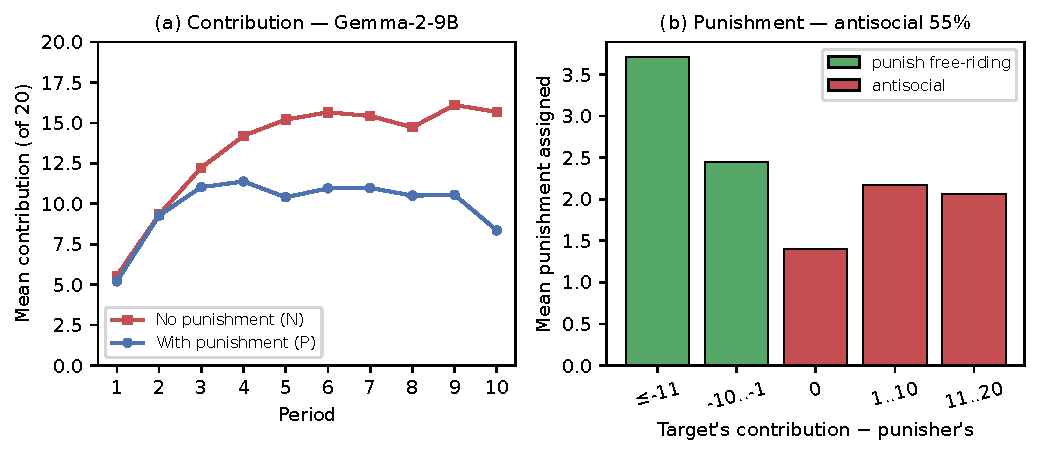
\includegraphics[width=0.80\textwidth]{fig1_punishment.pdf}\\[0.38em]
  {\small\textbf{\textcolor{accent}{Đường P nằm DƯỚI N — trừng phạt không nâng (Gemma còn giảm), ngược hẳn người.}}}\\[0.26em]
  {\footnotesize\color{mute}P$-$N $=$ \hlr{$-0.36 / -3.55 / +0.08$} vs người \hlg{$+4.3$}$^\dagger$ \;\textbullet\; TOST $p=.010/.002$ \;\textbullet\; $\mathrm{BF}_{01}$ 2.3/2.5}\\[0.12em]
  {\scriptsize\color{mute}$^\dagger$ mức tăng $+4.3$ của người là \emph{within-subject} (agent chơi N, P ở nhóm độc lập); (b) chỉ Gemma giữ gradient.}
\end{frame}

\begin{frame}{\pB{B3} — Cấu trúc xuyên văn hóa sụp đổ}
  \centering
  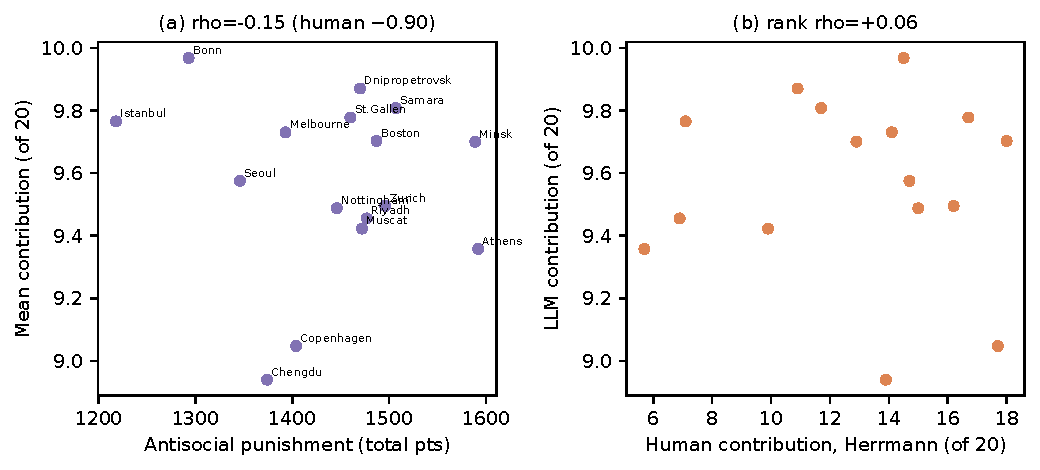
\includegraphics[width=0.82\textwidth]{fig2_cross.pdf}\\[0.4em]
  {\small\textbf{\textcolor{accent}{Liên kết antisocial--hợp tác $\rho\approx-0.90$ ở người $\to$ gần BẰNG 0 ở model; ``geography'' biến mất.}}}\\[0.28em]
  {\footnotesize\color{mute}$\rho=$ \hlr{$-0.09 / -0.15 / +0.30$} (người $-0.90$; Fisher-$z$ $p\le.0011$) \;\textbullet\; rank $\rho$ vs người $+0.33 / +0.06 / +0.17$}
\end{frame}

%% ================= SECTION 4 : SYNTHESIS =================
\section{Tổng hợp \& Kết luận}

\begin{frame}{Một tiêu chí, hai dissociation song song}
  \centering
  \renewcommand{\arraystretch}{1.45}
  \begin{tabular}{>{\raggedright\arraybackslash}p{0.20\textwidth} >{\raggedright\arraybackslash}p{0.36\textwidth} >{\raggedright\arraybackslash}p{0.36\textwidth}}
    \toprule
    & \hlg{Bề mặt được tái tạo} & \hlr{Cấu trúc chẩn đoán bị mất}\\
    \midrule
    \pA{Paper A}\newline CRSD / Climate & Hợp tác cao, đạt target 100\% & Phản ứng với \emph{loss probability} (vô cảm rủi ro)\\
    \midrule
    \pB{Paper B}\newline PGG / Punishment & Góp hào phóng + trừng phạt (54--59\% antisocial) & (i) trừng phạt nâng hợp tác; (ii) cấu trúc xuyên văn hóa\\
    \bottomrule
  \end{tabular}

  \vspace{0.5cm}
  \begin{block}{Mẫu hình chung}
    \centering
    ``Cooperation is \hlg{real as output}, \hlr{absent as mechanism}.'' — bề mặt giống người \emph{không} bảo chứng cho cơ chế giống người.
  \end{block}
\end{frame}

%% ================= THANK YOU =================
\begin{frame}[plain,noframenumbering]
  \begin{tikzpicture}[remember picture,overlay]
    \fill[primary] (current page.south west) rectangle (current page.north east);
    \fill[amber] ([yshift=-3.2cm]current page.west) rectangle ([yshift=-3.4cm]current page.east);
  \end{tikzpicture}
  \vfill
  \begin{center}
    {\color{white}\Huge\bfseries Cảm ơn}\\[0.6em]
    {\color{white!75!primary}\large Câu hỏi \& thảo luận}
  \end{center}
  \vfill
\end{frame}

\end{document}
